\documentclass[11pt]{article}

\def\mainroot{ell_1}

\usepackage[top=1in, bottom=1in, left=1in, right=1in]{geometry}

\usepackage[compact]{titlesec}

\usepackage{xcolor}
\definecolor{pykeyword}{HTML}{000088}
\definecolor{pyidentifier}{HTML}{000000}
\definecolor{pystring}{HTML}{008800}
\definecolor{pynumber}{HTML}{FF4000}
\definecolor{pycomment}{HTML}{880000}

\usepackage{listings}
\lstset{language=Python,
	basicstyle=\ttfamily\small,
	tabsize=4,
	showstringspaces=false,
	keywordstyle=\color{pykeyword},
	identifierstyle=\color{pyidentifier},
	stringstyle=\color{pystring},
	numberstyle=\color{pynumber},
	commentstyle=\color{pycomment}
}

\usepackage{algorithm}
\usepackage{algpseudocode}

\usepackage{graphicx}

\usepackage{amsmath}

\title{CSE 537 Assignment 5 Report: ML Classifiers}

\author{
Remy Oukaour \\
	{\small SBU ID: 107122849}\\
	{\small \texttt{remy.oukaour@gmail.com}}
\and
Jian Yang \\
	{\small SBU ID: 110168771}\\
	{\small \texttt{jian.yang.1@stonybrook.edu}}
}

\date{Wednesday, December 9, 2015}

\raggedbottom

\begin{document}

\maketitle

\section{Introduction}

This report describes our submission for assignment 5 in the CSE 537 course on
artificial intelligence. Assignment 5 requires us to implement two kinds of
machine learning classifiers: a decision tree classifier for predicting credit
worthiness of applicants, and a na{\"i}ve Bayes classifier for classifying
handwritten digits. In this report, we discuss the implementation details and
performance of our solutions.

\section{Decision tree classifier}

Jian Yang developed the decision tree classifier for predicting credit worthiness
of applicants.

% TODO

\section{Na{\"i}ve Bayes classifier}

Remy Oukaour developed the na{\"i}ve Bayes classifier for classifying handwritten
digits.

\subsection{Instructions}

To run the classifier, enter $python naive-bayes.py$. It will read from
$trainingimages.txt$, $traininglabels.txt$, $testimages.txt$, and $testlabels.txt$,
and output to $predictedlabels.txt$ and $confusion-matrix.txt$.

\subsection{Implementation}

The classifier is a straightforward implementation of na{\"i}ve Bayes, using the formula
``log posterior $\propto$ log prior + log likelihood'':

$$\log P(label|features) \propto \log P(label) + \sum_{feature} P(feature|label)$$

The prior probability $P(label)$ is estimated to be the fraction of training instances
with a given label (0 to 9). The likelihood of a feature having a certain value for a test
instance is estimated to be the fraction of training instances with that value for that
feature. (We use Laplace smoothing to handle novel feature values in the test data,
with a smoothing value of 0.001.) We then pick the label of each test instance using a
maximum likelihood estimator:

$$classification(features) = \underset{labels}{\operatorname{argmax}} \ \log P(label|features)$$

\subsection{Feature selection}

\subsection{Parameter tuning}

\subsection{Performance results}

\begin{figure}[h!]
\centering
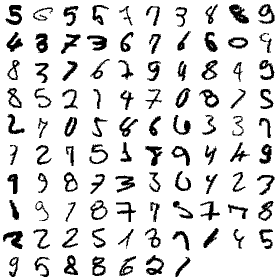
\includegraphics[height=2.75in, width=2.75in]{digits.png}
\caption{The 97 digits which the algorithm misclassified.}
\label{nbc_digits}
\end{figure}

\end{document}
